        \subsection{Monocromatizar Infinito}
            \subsubsection{Implementación ANSI-C (SISD)}
                Esta implementación es análoga a la de Monocromatizar Uno, solo que en vez de storear el resultado de una operación, calculamos el máximo de los 3 valores RGB correspondientes. Se procesa de un píxel a la vez. 
            \subsubsection{Implementación ASSEMBLER (SIMD)}
                El método para cargar las cosas en memoria es similar al de Gris Epsilon Uno también. Solo que el valor G se carga una sola vez (Es decir, en el primer byte de XMM0 queda B, en el primer byte de XMM1 queda G y en el primer byte de XMM2 queda R). Luego usando la instrucción PMAXUB obtenemos el valor máximo de cada byte entre esos registros y los dejamos en XMM0, como se ve en las imágenes.
                
                \begin{figure}[htb]
                \begin{center}
                \leavevmode
                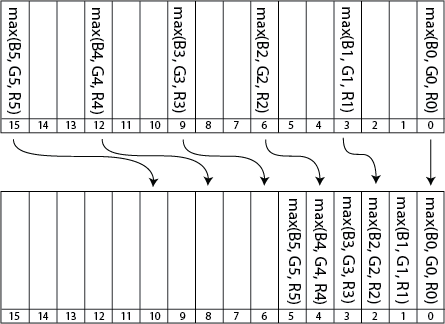
\includegraphics[width=0.5\textwidth]{gris_epsilon_infinito_pshub.png}
                \end{center}
                \caption{pshufb para acomodar los resultados}
                \end{figure}
                
                Luego, hacemos un PSHUFB para poder ordenar los valores de una forma que nos resulte cómoda para pasarlos a memoria, borrando los datos que no nos sirven. No hay problema al usar PSHUFB porque al no haber ni sumas ni restas no tenemos que saturar nada. El método para copiar a memoria es igual al de Monocromatizar Uno.

        \subsubsection{Comparación de Performance (SISD v SIMD)}

Acá va la comparación de performance entre C y ASM
